\documentclass[
  twoside,
  11pt, a4paper,
  footinclude=true,
  headinclude=true,
  cleardoublepage=empty
]{scrreprt}

\usepackage{lipsum}
\usepackage[utf8]{inputenc}
\usepackage[ngerman,english]{babel}
\usepackage{amsmath}
\usepackage{amsthm}
\usepackage{graphicx}
\usepackage{listings}
\usepackage{lmodern}
\usepackage{float}
\usepackage{sidecap}
\usepackage{acronym}
\usepackage{setspace}
\usepackage[customcolors]{hf-tikz}
\usepackage{url}
\usepackage{csquotes}
\usepackage[T1]{fontenc}
\graphicspath{ {images/} }

\begin{document}

\begin{titlepage}
    \begin{center}
        \Huge
        \textbf{Feasibility Study of Real Time Path Tracing}
        
        \vspace{0.5cm}

        \LARGE
        \textit{Or:} How Much Noise Is Too Much?
        
        \vspace{1.5cm}
        
        \textbf{Sven-Hendrik Haase}
        
        \vfill
        
        A thesis presented for the degree of\\
        \emph{Bachelor of Computer Science}
        
        \vspace{0.8cm}
        
        
\includegraphics[width=0.4\textwidth]{frontbackmatter/logo_uhh.jpg}
        
        % I was not allowed to use the old logo :( But I have much like it so I'm
        % keeping this here.
        %
\includegraphics[width=0.4\textwidth]{frontbackmatter/uni-siegel.png}
        
        \Large
        Department of Informatics\\
        University of Hamburg\\
        Germany\\
        2015-20-08

        \vspace{0.8cm}

        \large
        Primary Supervisor: Prof. Dr. rer. nat. Leonie \textsc{Dreschler-Fischer}\\
        Secondary Supervisor: Prof. Dr. Thomas \textsc{Ludwig}
        
    \end{center}
\end{titlepage}


\chapter*{Abstract}
\onehalfspace
This study aims to investigate the viability of a physically-based technique called
\textbf{path tracing} in lieu of or in corporation with classical techniques in interactive media
such as video games and visual effects tools.

Real time path tracing has been prohibitively expensive in regards to computational complexity.
However, modern \acs{gpu}s and even \acs{cpu}s have finally gotten fast enough for real time path
tracing to become a viable alternative to traditional real time approaches to rendering.  Based on
that assumption, this thesis presents the idea, algorithm and complexity behind path tracing in the
first part and extrapolates feasibility and suitability of real time path tracing on consumer
hardware according to the current state of technology and trends in the second part.

As part of the research, the author has implemented a path tracing 3D engine in modern C++ in order
to empirically test the assumptions made in this thesis. The study found path tracing to be a
viable rendering technique for average commodity hardware in approximately 4 years.
\singlespace

\chapter*{Acknowledgments}
\doublespacing
I would like to express my sincere gratitude to the teachers throughout school and university for
the knowledge they've passed on.

I thank my friends for the laughs, horrible mistakes and awesome successes we shared with
one another.

Furthermore, none of this would have been possible without the incredible efforts and love of my
parents who have supported me throughout the years and enabled me to live a carefree life until I
was ready to fend for myself.

Lastly, but certainly not least, I would like to declare my gratefulness to Alisa, whose endless love
has given my life a new meaning.

\singlespace

\clearpage
\vspace*{\fill}
\thispagestyle{empty} % suppress showing of page number
\begin{quotation}
    \em
    We all make choices in life, but in the end, our choices make us.

    \medskip
    \raggedleft
    Andrew Ryan
\end{quotation}
\vspace*{\fill}

\tableofcontents

\chapter*{Acronyms}
\begin{acronym}
    \acro{aabb}[AABB]{axis-aligned bounding box}
    \acro{ao}[AO]{ambient occlusion}
    \acro{brdf}[BRDF]{bidirectional reflection distribution function}
    \acro{bsp}[BSP]{binary space partitioning}
    \acro{cpu}[CPU]{central processing unit}
    \acro{csg}[CSG]{constructive solid geometry}
    \acro{fps}[FPS]{frames per second}
    \acro{gi}[GI]{global illumination}
    \acro{gpu}[GPU]{graphics processing unit}
    \acro{hdr}[HDR]{high dynamic range}
    \acro{mlt}[MLT]{Metropolis light transport}
    \acro{pbr}[PBR]{physically based rendering}
    \acro{rt}[RT]{real time}
    \acro{rgb}[RGB]{red-green-blue}
    \acro{simd}[SIMD]{single instruction multiple data}
    \acro{spp}[SPP]{samples per pixel}
    \acro{ssao}[SSAO]{screen-space ambient occlusion}
\end{acronym}

\chapter{Introduction}
As part of the quest for ever-improving game graphics, researchers, graphics hardware developers
and video game developers alike have been coming up with more and more convoluted and technically
challenging ways of improving the graphics in interactive media such as games and visualizations in
order to give users a deeper sense of immersion or to provide special effects artists with faster
feedback.

While rendering techniques are currently shifting from the traditional fixed pipeline approach
towards the new, fully programmable approach that lets developers implement deferred renderers that
can more closely mimic reality by using multiple combined shading and lighting algorithms and
rendering the scene multiple times for different buffers, the fundamental concept of
rasterization-based rendering has largely remained the same.

The real world photon-collecting approach that actual cameras use has so far not been adopted for
interactive media by the industry in any capacity because the computational cost has historically
been prohibitively expensive. It is, however, used extensively (and has been in use since decades)
for offline, non-interactive rendering of computer-generated movies and visualizations of
scientific simulations.

This study assumes that the next logical step for the industry will be to adopt this method for
real time media as well. For the purpose of this thesis, a renderer is considered
\textit{real time} when it manages to render a frame within \(16.67ms\) since that equals 60
\ac{fps} which is
the current de facto standard refresh rate for most available computer screens. Conversely, a
renderer is called \textit{offline} when it is not designed for interactive rendering which usually
means that it will renderer an image or a batch of images over the course of a few days. The
differences of real time and offline path tracing renderers will be explained in the next chapter.

\section{Motivation}
Real time path tracing (and physically based rendering in general) offers many
benefits over traditional real time rendering methods such as better visuals
and simpler implementation but also allows for completely new types of graphics
such as realistic caustics \cite{wiki:caustics} and even light dispersion
\cite{wiki:dispersion} (using a prism, for instance) since path tracers might simulate wavelengths
instead of plain \ac{rgb} colors. Modern video games tend
to rely on a growing number of tricks to keep them visually appealing as the
consumer grows more demanding. They're called \textit{tricks} in this study
because they merely trick the beholder into seeing something that appears to be
physically accurate when it is, in fact, not the result of a physically-based
calculation and as such this study aims to keep tricks and emergent phenomena
separated by language. Some notable tricks include \ac{ssao}
\cite{wiki:ssao}, motion blur \cite{wiki:motion-blur}, lens flares
\cite{wiki:lens-flare}, chromatic aberration \cite{wiki:chromatic-aberration},
depth of field \cite{wiki:depth-of-field} and light mapping \cite{wiki:lightmap}.

\chapter{Real Time Path Tracing Explained}
This chapter will explain the concepts, mathematics, physics and algorithms behind path tracing,
how real time path tracing differs from offline path tracing and the trade-offs made to achieve
acceptable performance. It will also explain how path tracing differs from rasterization and other
global illumination techniques.

\section{Physically Based Approach}
In our physical world, we see pictures because our eyes collect photons emitted by light
sources which then bounce around various surfaces until they eventually hit our eyes'
photoreceptor cells. On every bounce, a bit of light is absorbed which is why light loses intensity
when it bounces. Some surfaces absorb a particular band of wavelengths of the light when it bounces
which we perceive as a change in the light's color. Cameras work exactly like this as far as
collection of photons is concerned.

This physical approach would be extremely wasteful and
computationally complex to simulate, however, since most photons never reach an observer. Consider,
for instance, that only an extremely small percentage of all the photons sent by the Sun actually
reach Earth and an even smaller percentage of those are ever observed (although photons
don't have to be observed to have a physical effect, of course). Since we only care for photons that
are relevant to the image that we are trying to render, it makes more sense to use
\emph{backwards ray tracing} in which rays (which simulate streams of photons) are shot from the
observer into the scene for every sensor. It is called \textit{backwards} because the rays go
the reverse direction compared to their physical counterparts.

This is efficient since we usually only care about a
single observer (the scene camera) for which we will trace every single ray that it can possibly
perceive. In computer graphics terms, we will trace a ray for every pixel of the camera (and for
now we will assume that the viewport is exactly the same resolution as the camera simplicity's
sake). For every ray, we check for intersections with geometry and then either bounce a few more
times or shoot directly towards a light. We might do this multiple times per pixel to improve image
quality. This is called \emph{sampling}. The more iterations we spend on sampling, the better the
quality of our image becomes. This is called \emph{converging}.
There are a few approaches that improve on this such as bidirectional path tracing
\cite{techreport:pbr} and the \ac{mlt} \cite{inproceedings:metropolis}.

\section{Theoretical Basis}
\subsection{The Rendering Equation}
The fundamental problem solved by path tracing is the \emph{rendering equation} originally
described by James Kajiya \cite{inproceedings:pathtracing}. This thesis uses the form from
Wikipedia \cite{wiki:rendering-equation} since the author considers it easier to read:

\[
        L_{\text{o}}(\mathbf x,\, \omega_{\text{o}},\, \lambda,\, t) \,=
        \, L_{\text{e}}(\mathbf x,\, \omega_{\text{o}},\, \lambda,\, t) \ +
        \, \int_\Omega f_{\text{r}}(\mathbf x,\, \omega_{\text{i}},\ \omega_{\text{o}},\, \lambda,\, t)
        \, L_{\text{i}}(\mathbf x,\, \omega_{\text{i}},\, \lambda,\, t)\,
        (\omega_{\text{i}}\,\cdot\,\mathbf n)\, \operatorname d \omega_{\text{i}}
\]

For our purposes, this can be simplified by removing the time and wavelength components which we
will not make use of:

\[
        L_{\text{o}}(\mathbf x,\, \omega_{\text{o}}) \,=
        \, L_{\text{e}}(\mathbf x,\, \omega_{\text{o}}) \ +
        \, \int_\Omega f_{\text{r}}(\mathbf x,\, \omega_{\text{i}},\ \omega_{\text{o}})
        \, L_{\text{i}}(\mathbf x,\, \omega_{\text{i}})\,
        (\omega_{\text{i}}\,\cdot\,\mathbf n)\, \operatorname d \omega_{\text{i}}
\]

This equation can be broken down into its individual parts to make it easier to explain and
understand:

\[
        \tikzmarkin[set fill color=red!50!brown!30,set border color=red!40!black]{outgoing}
            L_{\text{o}}(\mathbf x,\, \omega_{\text{o}})
        \tikzmarkend{outgoing}
        \, = \,
        \tikzmarkin[set fill color=cyan!70!lime!30,set border color=cyan!40!black]{emitted}
        L_{\text{e}}(\mathbf x,\, \omega_{\text{o}})
        \tikzmarkend{emitted}
        \ + \,
        \tikzmarkin[set fill color=yellow!50!lime!30,set border color=yellow!40!black]{integral}(0.1,-0.4)(-0.1,0.6)
            \int_\Omega
        \tikzmarkin[set fill color=green!50!lime!30,set border color=green!40!black]{brdf}(0.0,-0.2)(-0.0,0.4)
            f_{\text{r}}(\mathbf x,\, \omega_{\text{i}},\ \omega_{\text{o}})
        \tikzmarkend{brdf}
        \,
        \tikzmarkin[set fill color=blue!50!lime!30,set border color=blue!40!black]{incoming}(0.0,-0.2)(-0.0,0.4)
            L_{\text{i}}(\mathbf x,\, \omega_{\text{i}})
        \tikzmarkend{incoming}
        \,
        \tikzmarkin[set fill color=magenta!100!lime!30,set border color=pink!40!black]{attenuation}(0.0,-0.2)(-0.0,0.4)
            (\omega_{\text{i}}\,\cdot\,\mathbf n)
        \tikzmarkend{attenuation}
        \,
            \operatorname d \omega_{\text{i}}
        \tikzmarkend{integral}
\]

\noindent
\(
        \tikzmarkin[set fill color=red!50!brown!30,set border color=red!40!black]{outgoing'}(0.1,-0.15)(-0.1,0.35)
        L_{\text{o}}(\mathbf x,\, \omega_{\text{o}})
        \tikzmarkend{outgoing'}
\)\, is the \textbf{outgoing light} with \(\mathbf x\) being a point on a surface from which the light is
reflected from into direction \(\omega_{\text{o}}\).

\noindent
\(
        \tikzmarkin[set fill color=cyan!70!lime!30,set border color=cyan!40!black]{emitted'}(0.1,-0.15)(-0.1,0.35)
        L_{\text{e}}(\mathbf x,\, \omega_{\text{o}})
        \tikzmarkend{emitted'}
\)\, is the \textbf{emitted light} from point \(\mathbf x\). Usually surfaces don't emit light themselves unless
they are area lights.

\noindent
\(
        \tikzmarkin[set fill color=yellow!50!lime!30,set border color=yellow!40!black]{integral'}(0.1,-0.2)(-0.1,0.35)
        \int_\Omega \, \ldots \, \operatorname d \omega_{\text{i}}
        \tikzmarkend{integral'}
\)\, is the integral over \(\Omega\) which is the hemisphere at \(\mathbf x\) (and thusly
centered around \(\mathbf n\)). All possible values for \(\omega_{\text{i}}\) are therefore
contained in \(\Omega\).

\noindent
\(
        \tikzmarkin[set fill color=green!50!lime!30,set border color=green!40!black]{brdf'}(0.1,-0.15)(-0.1,0.35)
            f_{\text{r}}(\mathbf x,\, \omega_{\text{i}},\ \omega_{\text{o}})
        \tikzmarkend{brdf'}
\)\, is the \textbf{\ac{brdf}} which determines how much light is reflected from
\(\omega_{\text{i}}\) to \(\omega_{\text{o}}\) at \(\mathbf x\).

\noindent
\(
        \tikzmarkin[set fill color=blue!50!lime!30,set border color=blue!40!black]{incoming'}(0.1,-0.15)(-0.1,0.35)
            L_{\text{i}}(\mathbf x,\, \omega_{\text{i}})
        \tikzmarkend{incoming'}
\)\, is the \textbf{incoming light} at \(\mathbf x\) from \(\omega_{\text{o}}\). It is not necessarily
\emph{direct light}. The rendering equation also considers \emph{indirect light} which is light that has already
been reflected.

\noindent
\(
        \tikzmarkin[set fill color=magenta!100!lime!30,set border color=pink!40!black]{attenuation'}(0.1,-0.15)(-0.1,0.35)
            (\omega_{\text{i}}\,\cdot\,\mathbf n)
        \tikzmarkend{attenuation'}
\)\, is the \textbf{normal attenuation} at \(\mathbf x\). The incoming light \(\omega_{\text{i}}\) is
weakened depending on the cosine of the angle between \(\omega_{\text{i}}\) and the surface normal
\(\mathbf n\).
\\

Path tracing offers a numerical solution to the integral found in this equation. For every pixel,
every bounce and every sample of the camera, the rendering equation is solved. It becomes apparent
why this is an expensive algorithm to run. For practical reasons, not every possible value for
\(\Omega\) is sampled since this would take a vast amount of time to calculate at physical photon
density. Instead, only a few possible values for \(\Omega\) are calculated each bounce. Depending
on the exact algorithm used, usually only a low number of samples (approximately 20) is required for the
image to converge to an acceptable level of quality.

\subsection{Algorithm}
Python-like pseudocode:
\begin{lstlisting}[language=Python]
max_depth = 5

def trace_ray(ray, depth):
    if depth >= max_depth:
        # Return black since we haven't hit anything but we're
        # at our limit for bounces
        return RGB(0, 0, 0) 

    collision = ray.check_collision()
    if not collision:
        # If we haven't hit anything, we can't bounce again so
        # we return black
        return RGB(0, 0, 0)

    material = collision.material;
    emittance = material.emittance # kill this

    # shoot a ray into random direction and recurse
    next_ray = Ray()
    next_ray.origin = collision.position
    next_ray.direction = random_vector_on_hemisphere(collision.normal)

    reflectance_theta = dot(next_ray.direction, collision.normal)
    brdf = 2 * material.reflectance * reflectance_theta
    reflected = trace_ray(next_ray, depth + 1)

    return emittance + (brdf * reflecte)

for pixel in pixels:
    trace_path(pixel)
\end{lstlisting}


\section{Properties of Path Tracing}
Advantages and Disadvantages blah

\subsection{Comparison to Traditional Ray Tracing}

\subsection{Comparison to Rasterization}

\subsection{Comparison to Other Algorithms}

\section{History of Path Tracing}
As with so many things in computer science and science in general, the modern idea of physically
based rendering using path tracing builds upon many important past discoveries and algorithms
such as ray tracing and ray casting.
Arthur Appel is generally credited as being the father of
\emph{ray casting} as he was the first to describe the algorithm in a 1968 paper
\cite{inproceedings:raycasting}.

Ray casting is an important idea needed for \emph{ray tracing} which was
first published in a paper in 1980 by Turner Whitted \cite{article:raytracing}.

\begin{figure}[h]
    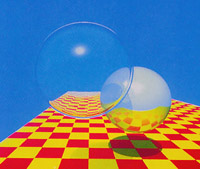
\includegraphics{early-raytracing-whitted}
    \centering
    \caption{Turner Whitted's original 1980 \cite{article:raytracing} image showing off the usage of ray tracing for
    reflection, refraction and shadows.}
    \label{fig:early-raytracing-whitted}
\end{figure}
Building upon ray tracing, an improved algorithm was published in 1986 by James T. Kajiya which used ray tracing
combined with a Monte Carlo algorithm in order to create a new algorithm that was called \emph{Monte
Carlo ray tracing} \cite{inproceedings:pathtracing}. Nowadays, Monte Carlo ray tracing is better
known as \emph{path tracing}.

It took another decade for path tracing to become the
physically based rendering approach that it is known for today. In 1996, Eric Lafortune improved
the algorithm by suggesting the usage of bidirectional path tracing \cite{techreport:pbr} and
finally the \ac{mlt} was suggested in 1997 by Eric Veach and Leonidas J. Guibas \cite{inproceedings:metropolis} to
improve performance in complex scenes.

This was the last notable improvement to the algorithm,
though many micro optimizations have since been published. All of these achievements and
improvements are generally collapsed into the term \emph{path tracing} since they do not diverge
from the general algorithm but instead improve upon it.

It took longer still for the industry to become interested in path tracing. The early interest in
ray tracing was of mostly academical and recreational nature. One of the most notable creations of
the early days of ray tracing is The Juggler created and published by Eric Graham in 1986
\cite{site:juggler} on an Amiga 1000. It was a pre-rendered animation using ray tracing. Eric Graham
stated that it took the Amiga 1 hour to render each frame \cite{site:juggler}.

\begin{figure}[H]
    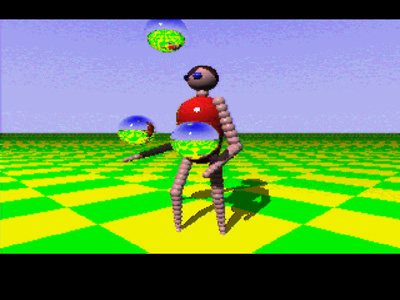
\includegraphics[scale=0.5]{amiga-juggler}
    \centering
    \caption{Eric Graham's Juggler}
    \label{fig:amiga-juggler}
\end{figure}
While the animation seems very primitive compared to the animations of today, it was exceptional at
the time. Ernie Wright's statement about The Juggler provides some contemporary context:

\blockquote[\cite{site:juggler}]{Turner Whitted's paper (1980) is widely regarded as the first modern
description of ray tracing methods in computer graphics. This paper's famous image of balls floating
above a checkerboard floor took 74 minutes to render on a DEC VAX 11/780 mainframe, a \$400,000
computer. The Juggler would appear a mere six years later, created and displayed on a \$2000 Amiga.}

The first feature-length computer-animated film,
\textit{Toy Story}, released in 1995 \cite{wiki:toy-story}, is sometimes miscredited as being the
first film using a ray tracing-like algorithm. However, it actually used traditional scanline
rendering. The first feature-length film using ray tracing, \textit{Cars}, was released much later,
in 2006 \cite{wiki:cars} \cite{inproceedings:cars} and started a wave of interest in the movie industry.

The first example of \emph{real time} path tracing was likely produced by the demo scene
\cite{wiki:demoscene} which was quick to adopt it \cite{site:realtime-radiosity-demos}
for the purpose of producing complex graphics rendered and generated on the fly. One notable
example of this is the WebGL Path Tracing by Evan Wallace made in 2010
\cite{site:webgl-path-tracing} which runs in most modern web browsers, making path tracing very
accessible.

\begin{figure}[H]
    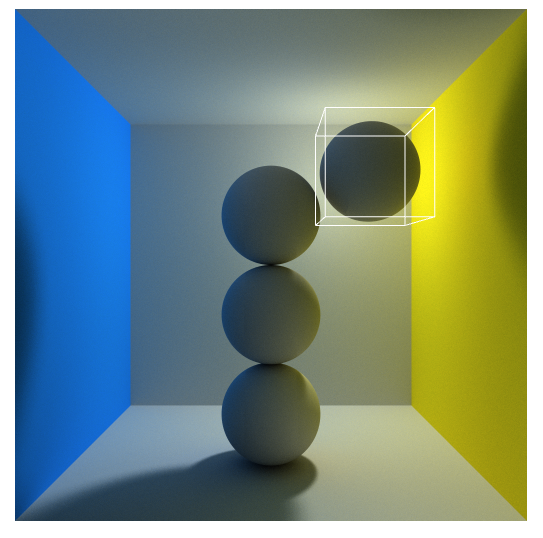
\includegraphics[scale=0.4]{webgl-pathtracer}
    \centering
    \caption{WebGL Path Tracer by Evan Wallace}
    \label{fig:webgl-pathtracer}
\end{figure}

Another example is the demo \textit{5 faces} by Fairlight from 2013
\cite{wiki:5faces-fairlight} which
uses a real time ray tracer running on the \acs{gpu} to render a complex scene at 30 \acs{fps}.

\begin{figure}[H]
    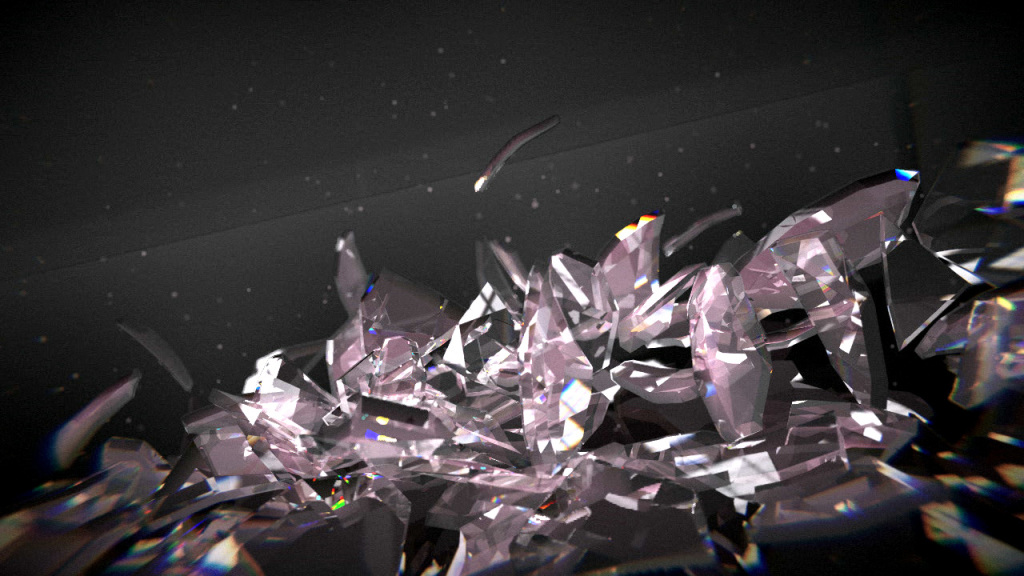
\includegraphics[scale=0.5]{5faces}
    \centering
    \caption{5 faces by Fairlight}
    \label{fig:5faces}
\end{figure}

In the past, some critics have offered critical insights about why it might not be a viable
alternative to rasterization on consumer hardware in the short
term \cite{site:raytracing-vs-rasterization} \cite{site:codinghorror-raytracing}.

\section{Current State of Technology}
lol
\lipsum[1]

\chapter{Research}
\lipsum[1]

\section{Results}
\lipsum[1]

\section{Evaluation}
\lipsum[1]

\chapter{Conclusion}
\lipsum[1]

\section{Outlook}
\lipsum[1]

\listoffigures
 
\listoftables

\bibliographystyle{unsrt}
\bibliography{main}
    
\end{document}
